\documentclass[12pt]{article}
\usepackage[utf8]{inputenc}
\usepackage{amsmath}
\usepackage{graphicx}
\usepackage{hyperref}
\usepackage{geometry}
\geometry{margin=1in}

\title{Algorithms: Design and Analysis \\ Checkpoint 2}
\author{
  Team 53 \\
  Members: Qurba Mushtaq, Hiba Shahid
}
\date{}

\begin{document}

\maketitle

\noindent\textbf{Reviewed research paper title:} \\
\textit{Bidirectional Dijkstra's Algorithm is Instance-Optimal} \\
by Bernhad Haeupler, Richard Hladik, Vaclav Rozhon, Robert E. Tarjan

% \vspace{1em}
% \noindent\textbf{GitHub:} 
% \url{https://github.com/HibaShahidA/Bidirectional-Dijkstra}

\section*{Introduction-Problem and Contribution}
For any given graphs, the algorithm with the near-optimal time complexity for finding the shortest st-path is Dijkstra's algorithm. However, for much larger graphs, as seen in real world scenarios, there are other algorithms that perform far better. One of these algorithms is bidirectional search using the Dijkstra's algorithm. The way it is performed is through executing Dijkstra's algorithm from both endpoints (s and t) in parallel. 

In huge graphs, specifically (non-negative) weighted multigraphs - both directed and undirected - use of bidirectional search is instance-optimal with respect to the number of edges it explores. This is different from the general Dijkstra's algorithm that is executed by traversing through all paths to find the shortest one - exploring the entire input graph. 

Although the worst-case complexity remains the same, bidirectional search has an upper hand on the Dijkstra's algorithm - especially for unweighted graphs where it is instance-optimal up to a factor of O(delta) where delta is the maximum degree of the graph.

\section*{Algorithm}
Think of two people walking towards one another along the shortest - one from the source and one from the target. If both take the optimal steps and meet in the middle, neither has to walk the full path. Similarly, in the bidirectional search, the search path does not have to explore the entire input graph. 

\begin{figure}[h]
\centering
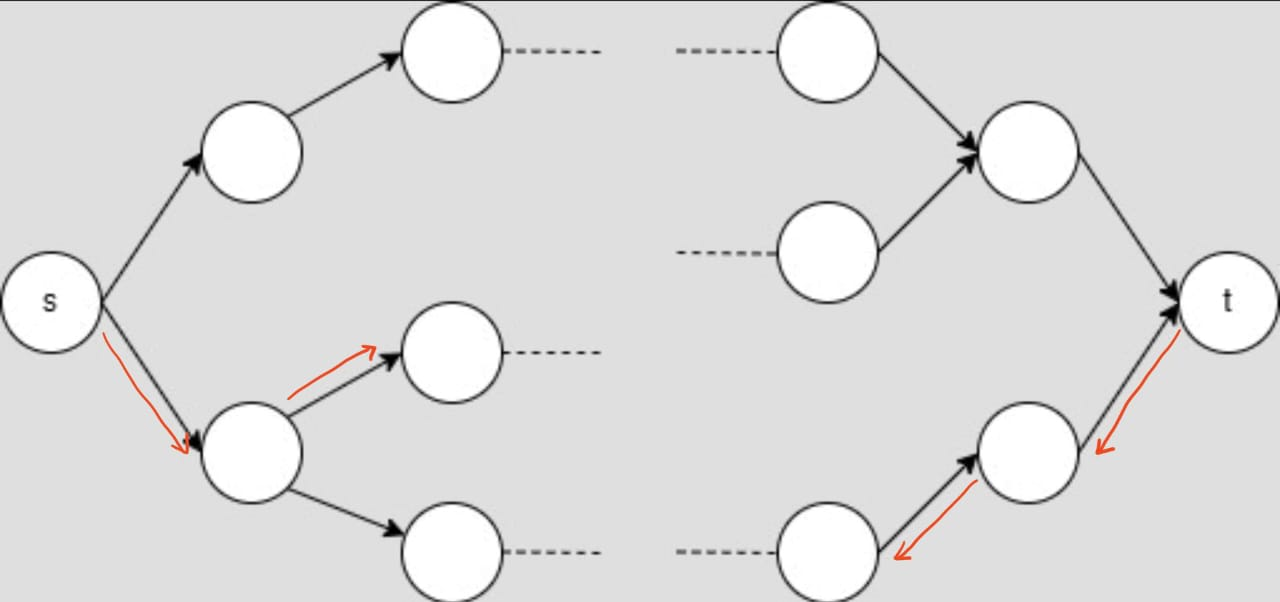
\includegraphics[width=0.8\textwidth]{BidirectionalDijkstra-cp2-edit.jpg}
\caption{The \textbf{red arrows} show the traversal that the algorithm takes. Irrespective of the direction of the edges, since the reverse traversal works similar to that of the forward traversal (much like residual graph traversal).}
\end{figure}

\noindent\textbf{Input:} The input of the algorithm is a graph \( G = (V, E) \) with non-negative edge weights, a source vertex \( s \) and a target vertex \( t \). \\
\textbf{Output:} The length and path of the shortest path from \( s \) to \( t \), if a path exists. \( \infty \) otherwise.

The input graph \( G \), each with a source vertex \( s \) and a target vertex \( t \), is traversed such that an optimal path search is started from \( s \) and an optimal path search is started from \( t \) simultaneously. Once the traversal from both endpoints meets, it is terminated - a path has been found.

\section*{Comparison}
The paper proves that Bidirectional Dijkstra's algorithm is instance-optimal (mathematically optimal for every individual input graph, not just in worst-case scenarios) for finding shortest paths in weighted graphs, meaning no correct algorithm can outperform it by more than a constant factor on any input. Unlike standard Dijkstra's algorithm, which explores outward from the source, bidirectional search runs two simultaneous Dijkstra executions (forward from s and backward from t).

Previous variants (Dantzig, Nicholson, Pohl) lacked instance-optimality guarantees due to two key flaws:

Their selection rules ("None of those approaches [Dantzig's alternation, Nicholson's closest-node, Pohl's queue-size] achieve the instance-optimality guarantees" - Theorem 1)

Their stopping conditions (Early versions used "a seemingly natural stopping condition that is not correct" - stopping at first intersection rather than path confirmation)

This work overcomes these limitations by introducing:

A strict alternation rule (one forward step, one backward step)

A correct stopping condition (ensures termination only when the shortest path is confirmed)

The result holds for both directed and undirected graphs with positive weights, while in unweighted graphs, the algorithm is optimal up to a factor of \( O(\Delta) \) (scales with the graph's maximum degree \( \Delta \)). Unlike A* (a heuristic-guided search that uses estimated distances to prioritize nodes), which relies on heuristics (problem-specific estimates to guide search), bidirectional Dijkstra is optimal without additional information, making it the best general-purpose shortest-path algorithm in this setting.

\section*{Data Structures and Techniques}
The algorithm traverses from both endpoints, and therefore, needs to maintain a list of visited nodes from both ends separately, along with two distance maps and two priority queues. 

\textbf{Initialization step:}
\begin{itemize}
  \item Create two priority queues \( Q_f \) and \( Q_b \); \( Q_f \) for forward search from \( s \), and \( Q_b \) for backward search from \( t \)
  \item Create two distance maps: \( d_f \) and \( d_b \), where \( d_f(s)=0 \) and \( d_b(t)=0 \) while all others are \( \infty \) (these are to track the distances and find the path)
  \item Create two visited sets \( S_f \) and \( S_b \) for forward search and backward search respectively
\end{itemize}

\textbf{Search step:}
This is an alternating approach between the forward and backward Dijkstra's. In each iteration, the algorithm picks the node with the smallest distance from either \( Q_f \) or \( Q_b \). For the forward direction, it pops the top of \( Q_f \), marks it visited in \( S_f \), and relaxes all its neighbors—updating distances in \( d_f \) and pushing better options into \( Q_f \). The same thing happens in the reverse direction using \( Q_b \) and \( d_b \) over the reversed graph, updating \( S_b \) as it goes. The search keeps going until a node gets marked visited by both sides—meaning the paths have met, and we can compute the shortest one using the sum of distances from both directions.

\textbf{Stopping conditions:}
If a node has been marked as visited in both the sets \( S_f \) and \( S_b \), then the search is stopped. Then, let 
\[
\mu = \min_{v \in S_f \cap S_b}(d_f(v) + d_b(v))
\]
be the shortest path found.

\textbf{Final output:} \\
Returns \( \mu \) as the length of the shortest path (or optionally, can also return the path alongside).

\section*{Time Complexity}
The worst-case is the same as the standard Dijkstra's algorithm: \( O((V+E)\log V) \) with binary heaps. Performance wise, however, it is much faster since each search explores roughly \( \sqrt{n} \) nodes in ideal setting reducing total work. It is important to note that in the worst-case scenario, where no shortest path (or any path) exists, will be equal to that of the Dijkstra's algorithm, since that would require exploring the entire graph. However, the average-case time complexity improves, since on average the number of nodes traversed is significantly smaller (\( \sqrt{n} \)).

\section*{Implementation outlook}
It is important that this algorithm be implemented carefully, since it has shown great potential for non-negative weighted graphs and unweighted as well. However, these may not work on negative weights, since much like the Dijkstra's algorithm that lacks the ability to find shortest path in a negative weighted graph, the bidirectional search approach lacks it as well. One way to tackle this issue would be to update the algorithm in a way that it acknowledges and gracefully handles the negative values. 

On the other hand, the improvement may show in huge graphs, therefore, the test would require very large input. Proper management of the heaps would also be required so as not to have any residual data or dangling pointers polluting the memory.

\section*{Additional Information}
To ensure thorough testing, we plan to begin with synthetic (automatically generated) graphs of varying sizes and properties. Once the algorithm performs reliably on these, we will test it on real-world datasets, such as the \textbf{Twitter} social network graph.

\section*{GitHub Repository}
\textbf{URL:} \url{https://github.com/HibaShahidA/Bidirectional-Dijkstra}\\


\end{document}

